%!Tex root = bare_conf.tex

\section{Evaluation}
We implemented MCTS for Da Vincicode upon 4-CPU(Pascal Titan Xp) and 12-core CPU.
We measured the execution time to analysis the dominant factor of time consuming.
We evaluated the performance and difference between \cpu and \gpu through measuring the number of simulation per second.

\subsection{Execution Time}
\begin{figure}
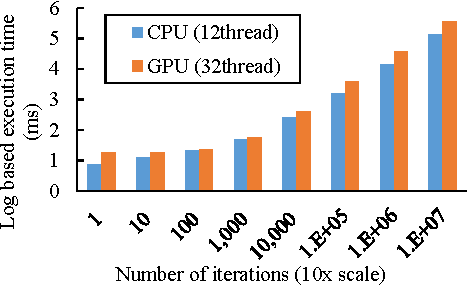
\includegraphics[width=0.95\columnwidth]{figures/time_consuming.pdf}
\caption{The time consuming according to the number of iterations}
\label{fig:time_consuming}
\end{figure}

We measured the execution time by varying the number of simulations from 1 to $10^7$ and calculated average values on 5 times execution. 
The \cref{fig:time_consuming} shows the execution time which was measured using 12 threads upon \cpu and using 32 threads upon \gpu.
We could observe that the execution time increases as the number of simulations increases.
Therefore, the number of simulation can be dominant factor of time consuming. 

The \cref{fig:time_consuming} shows that the execution is not much different when the number of simulations is small.
The memory access to the large array becomes the key factor of the performance when the number of simulation is small.
The number of simulations and the execution time are proportional as the number of simulations increases.
The computing becomes the key factor when the number of simulation is large.
Therefore, the performance (execution time) is proportional to the number of simulations, if amount of computation is large.

\subsection{The Number of Simulations per Second}
\subsubsection{CPU}
\begin{figure}
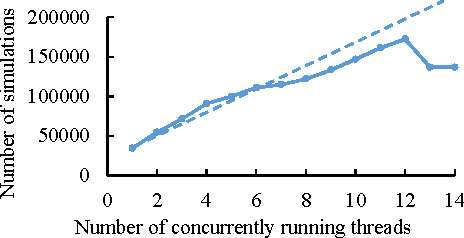
\includegraphics[width=0.95\columnwidth]{figures/cpu_num_simulation.pdf}
\caption{The number of simulations per second on CPU}
\label{fig:cpu_num_simulation}
\end{figure}

The \cref{fig:cpu_num_simulation} shows the result of the number of simulation per second over increasing number of threads of CPU. 
The number of simulations per second increases linearly.
However, the number of simulations decrease if the number of threads exceeds 12. 
The reason why the number of simulations decrease is that we have only 12 core. In other word, the number of physical cores is the scalability bootleneck. 
Therefore, it can be seen that the performance increases linearly with the number of cores in the CPU. 
\subsubsection{GPU}
\begin{figure}
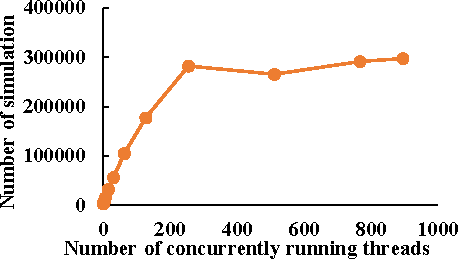
\includegraphics[width=0.95\columnwidth]{figures/gpu_num_simulation.pdf}
\caption{The number of simulations per second on GPU}
\label{fig:gpu_num_simulation}
\end{figure}

The \cref{fig:gpu_num_simulation} shows the result of the number of simulation per second over increasing number of threads of GPU. 
Unlike the \cref{fig:cpu_num_simulation}, the \cref{fig:gpu_num_simulation} shows the non-linear fashion. 
In addition, the graph has instant performance degradation at the middle despite increasing the number of threads. 
This is because cache misses increase as the number of thread is used, and memory bottlenecks from cache misses are higher than computaion performance obtained by increasing threads in GPU.

We measured the number of simulations with varying the number of warps to identify the valley which is mentioned in ~\cite{li2015priority_valley}. 
\begin{figure}
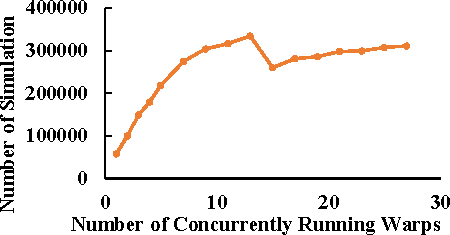
\includegraphics[width=0.95\columnwidth]{figures/gpu_warp_simulation.pdf}
\caption{The number of simulation according to the number of warps on GPU}
\label{fig:gpu_warp_simulation}
\end{figure}

The \cref{fig:gpu_warp_simulation} shows the result of experiment that measured the number of simulations according to the number of warps. 
If the number of warps is over 12, the performance decrease like ~\cite{li2015priority_valley}. 
The memory contention makes valley, therefore the the number of simulation reducte despite increasing the number of warps. 

\begin{figure}
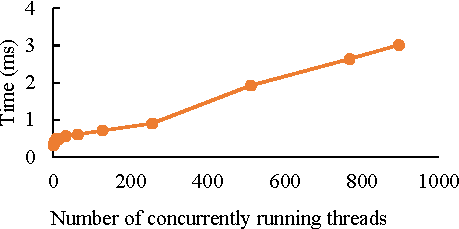
\includegraphics[width=0.95\columnwidth]{figures/gpu_thread_time.pdf}
\caption{How much time takes to execute application on GPU depending on thread size}
\label{fig:gpu_thread_time}
\end{figure}

In MCTS based on GPU, the threads which are already finished should wait until the thread which has the most number of turns ends. 
Because other threads need to wait for the longest thread, the MCTS based on GPU should be the weak scaling which takes the same amount of time to increase the number of threads.
However, the \cref{fig:gpu_thread_time} which shows that weak scaling is not sustained. 
There are two reasons why the \cref{fig:gpu_thread_time} is not weak scaling. 
First is path divergence issue until 16 threads. 
Many divergences to guess the opponent's tile take more time to finish compuation.   
Second is memory contention issue which performance valley as we mentioned previous more than 16 threads.
As the number of threads increases, not enough memory makes memory contention so the time takes more time.
